\documentclass[../main.tex]{subfiles} % required, if the Chapter be a seperate doc

\begin{document}

\chapter{Experimenteller Teil}\label{ch:experimenteller-teil}

    \section{Versuchsaufbau}\label{sec:versuchsaufbau}
    \subsection{Verwendete Materialien}\label{subsec:versuchsaufbau}
    % \begin{figure}[h]
    %     \centering
    %     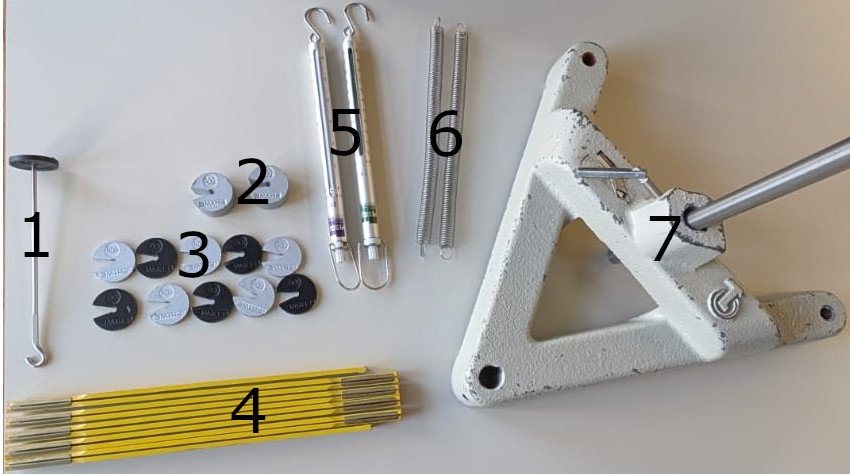
\includegraphics[width=1\textwidth]{Materialien}
    %     \label{fig:mesh1}
    % \end{figure}
    \begin{enumerate}
        \item TO-DO
        \item 2 X 50 g Gewichte Weiss
        \item 10 X 10 g Gewichte Weiss und Schwarz
        \item Doppelmeter
        % \item Newtonmeter 1 N und 10 N
        % \item 2 Federn
        % \item To-Do
    \end{enumerate}
    \begin{tcolorbox}[title=Hinweis zu den Gewichtsangeben]
        Die Genauigkeit von den Gewichtsangaben wurde von uns nicht kontrolliert. Es wurde uns aber gesagt, dass wir davon ausgehen können das diese Korrekt sind.
    \end{tcolorbox}
    \subsubsection{Genauere Beschreibung}\label{subsubsec:materialien}
    \text{Gewichte}

    \subsection{Aufbau}\label{subsec:aufbau}
    \text{Image to do}
    Als Grundlage dient ein Fuss der eine Stange hebt. Dies stange ist Senkrecht. 
    Die Länge oder Dicker der Stange ist egal. An die Stande kommt dann ein Stangenbefestigung. 
    Diese befestigt eine andere Stange, die senkrecht ist. 
    Die Breite der Stange ist soweit relevant, dass man die Feder daran besfestigen kan. Die Länge spielt keine Rolle.
    An der Stange ist eine Feder befestigt. Diese Feder ist mit dem TO-DO verbunden.
    An dem dann die Gewichte befestigt werden.
    Der Doppelmeter ist von Fuss bis zu der Stangenbefestigung anzubringen. Dabei sollte daruf geachtet werden, dass der Doppelmeter möglich gerade und parallel zur Stange ist.
    Am Doppelmeter sollte dann dazu dienen, abzulesen wie weit sich die Feder dehnt.

    \section{Durchführung}\label{sec:durchführung}
    
    \subsection{Methode zum ablesen der Werte auf dem Doppelmeter}\label{subsec:schritt-für-schritt-anleitung}

    Wenn in den unteren Texten von ablesen die Rede ist, dann ist folgendes gemeint:
    Alle 3 Gruppenteilnehmen Lesen den Wert unabhänig voneinander ab. Dann wird der Durchschnitt dieses Wertes genommen. Und dies gilt dann als der Wert, der abgelesen wurde.

    \begin{tcolorbox}[title=Hinweis beilm Ablesen]
        Die Werte wurden unabhänig voneinander abgelesen.
        Wenn eine zu grosse Differenzen zwischen den Werten war, also grösser als ein paar Millimeter, dann wurde der Wert nochmals abgelesen.
        Da man dann davon ausgehen konnte das es ein Ablesfehler gab.
    \end{tcolorbox}

    \subsection{Schritt für Schritt Anleitung}\label{subsec:schritt-für-schritt-anleitung}
    \begin{enumerate}
        \item Man Entfernt alles Gewicht von der Feder
        \item Man misst die länge der Feder.
        \item Man macht die gewünschte Gewichtung an die Feder.
        \item Man wiederholt die Schritte 2-3 bis man alle Gewichtungen gemacht hat.
    \end{enumerate}

    \subsection{Dinge die es zu beachten gibt}\label{subsec:dinge-die-es-zu-beachten-gibt}
    \text{
        Für die Länge einer Feder diehnt nur der Teil, der sich unter dem Gewicht auch ausdehnt. Das heisst die Kreise die oben und unten an der Feder angebracht sind zum sie befestigen gehören nicht zur Feder dazu.
        
    }


    
\end{document}